%!TEX root = ..\dissertation.tex
\chapter*{Curriculum Vitae}\markboth{Curriculum Vitae}{Curriculum Vitae}\label{chp:cv}
\addcontentsline{toc}{chapter}{Curriculum Vitae}
\begin{tabularx}{\textwidth}{@{}Xr}
    \LARGE\docAuthor~\href{https://orcid.org/0000-0001-9395-2411}{
\includegraphics[height=8pt]{frontmatter/figures/ORCIDiD_icon128x128}}&\raisebox{-\totalheight/2}{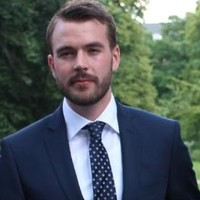
\includegraphics[width=4cm]{frontmatter/figures/cvPicture}}\\%Check up on DPI and make it round
\end{tabularx}\par\vspace{\baselineskip}\noindent
\docAuthor{} was born in Silkeborg, Denmark.
From 2011, he studied mechanical engineering at Aalborg University, receiving his \BSc{} in 2014, followed by a \MSc{} in manufacturing technology in 2016.
Since September 2016, he has been a \PhD{} fellow at Aalborg University's Department of Materials and Production as part of the Mass Customization research group.
During his \PhD{} studies, he stayed for three months as a visiting researcher at the Intelligent Manufacturing Systems Centre (IMSC) at the University of Windsor in Canada.
His research on manufacturing system platforms, their nature, development, documentation, and utilisation is part of the Manufacturing Academy of Denmark (MADE), funded by the Innovation Fund Denmark.
